\section{基本方程式}
\label{sec:core}

\paragraph{形式的範囲と未解決の仮定}
定義域、幾何と測度、パラメータの範囲は完全には指定されていない。
関連するIFGTの定式化にある追加の仮定や慣例は、正規化の選択も含め、CTへの特殊化条件として自動的には採用しない。
以下の範囲に関する記述は、欠けている仕様を示すものであり、それを補うものではない。

\subsection{場の発展}
ここでは収支関係を、モデルレベルの形式的テンプレートとして用いる。
定義域、初期条件・境界条件、正則性、正値性の保存条件を含む完全な初期境界値問題は指定していない。
この関係を用いることは、存在、一意性、適切性の確立を意味しない。
\begin{equation}
  \frac{\partial I}{\partial\tau} + \nabla\cdot\JI = \sigma,
  \label{eq:I_evolution}
\end{equation}
ここで情報流は
\begin{equation}
  \JI = -D\nabla I + \mu F_I, \qquad F_I = -\nabla\Phi = \alpha\nabla C,
  \label{eq:JI}
\end{equation}
である。力の関係において、最初の等号は負のポテンシャル勾配から有効力を定義する。
続く閉包勾配との等式は、局所的・有効な特殊化を意図したものであり、一般的な場の関係として保持する主要な畳み込みからの導出ではない。
この特殊化が有効となる近似領域と仮定は、今後確定する必要がある。

生成項は次のように分解する。
\begin{equation}
  \sigma = \sigma_{\mathrm{drive}} - \sigma_{\mathrm{dissip}} - \sigma_{\mathrm{barrier}}.
  \label{eq:sigma}
\end{equation}

三つの寄与は次のとおりである。
\begin{align}
  \sigma_{\mathrm{drive}}  &= a\Delta\!\left(1 - \frac{C}{C_*}\right),
  \label{eq:sigma_drive}\\
  \sigma_{\mathrm{dissip}} &= \Gamma C,
  \label{eq:sigma_dissip}\\
  \sigma_{\mathrm{barrier}}&= \frac{\kappa_B}{\Cmax - C}.
  \label{eq:sigma_barrier}
\end{align}

ここで$C_*$は観測窓内における概念的準閉包の有効飽和スケールを、$\Cmax$は理想的な完全閉包境界を表す。
概念的領域では一般に$C_* < \Cmax$である。

以下は有効な認知的解釈であり、測定された機構ではない。
$\sigma_{\mathrm{drive}}$は新たな入力（知覚、言語的摂動、報酬信号）の流入を表す。
$\sigma_{\mathrm{dissip}}$は未解決の緊張の自然な減衰（忘却、馴化）を表す。
$\sigma_{\mathrm{barrier}}$は概念的な過閉包に対する、投影的または粗視化された有効抵抗を表す。
これは基礎的な外部からの禁止として読むべきではなく、VEDとIFGTで用いられる有効障壁の記法に対する、認知領域での類似物である。
逆数の形だけでは、示された上側境界に動的に到達できないことは証明されない。
逆数表式の発散と全発展のもとでの不変性は別の主張であり、端点での振る舞いも不変領域の条件も、ここでは確立されていない。

\subsection{トークンと場の結合}
本構成では、離散的で再アドレス可能な構造を、安定で低コストな再帰のために提案する要件として扱う。
その動機は、連続場の配置を再訪することにはコストがかかり、ドリフトが生じやすい可能性にある。
連続系一般について不可能性を主張するものではない。
再アドレス可能性は、複雑な状態の再利用を支えることを意図している。
図\ref{fig:token-field-coupling}は結合仮説の例示であり、その帰結を実行によって示したものではない。

\begin{figure}[t]
\centering
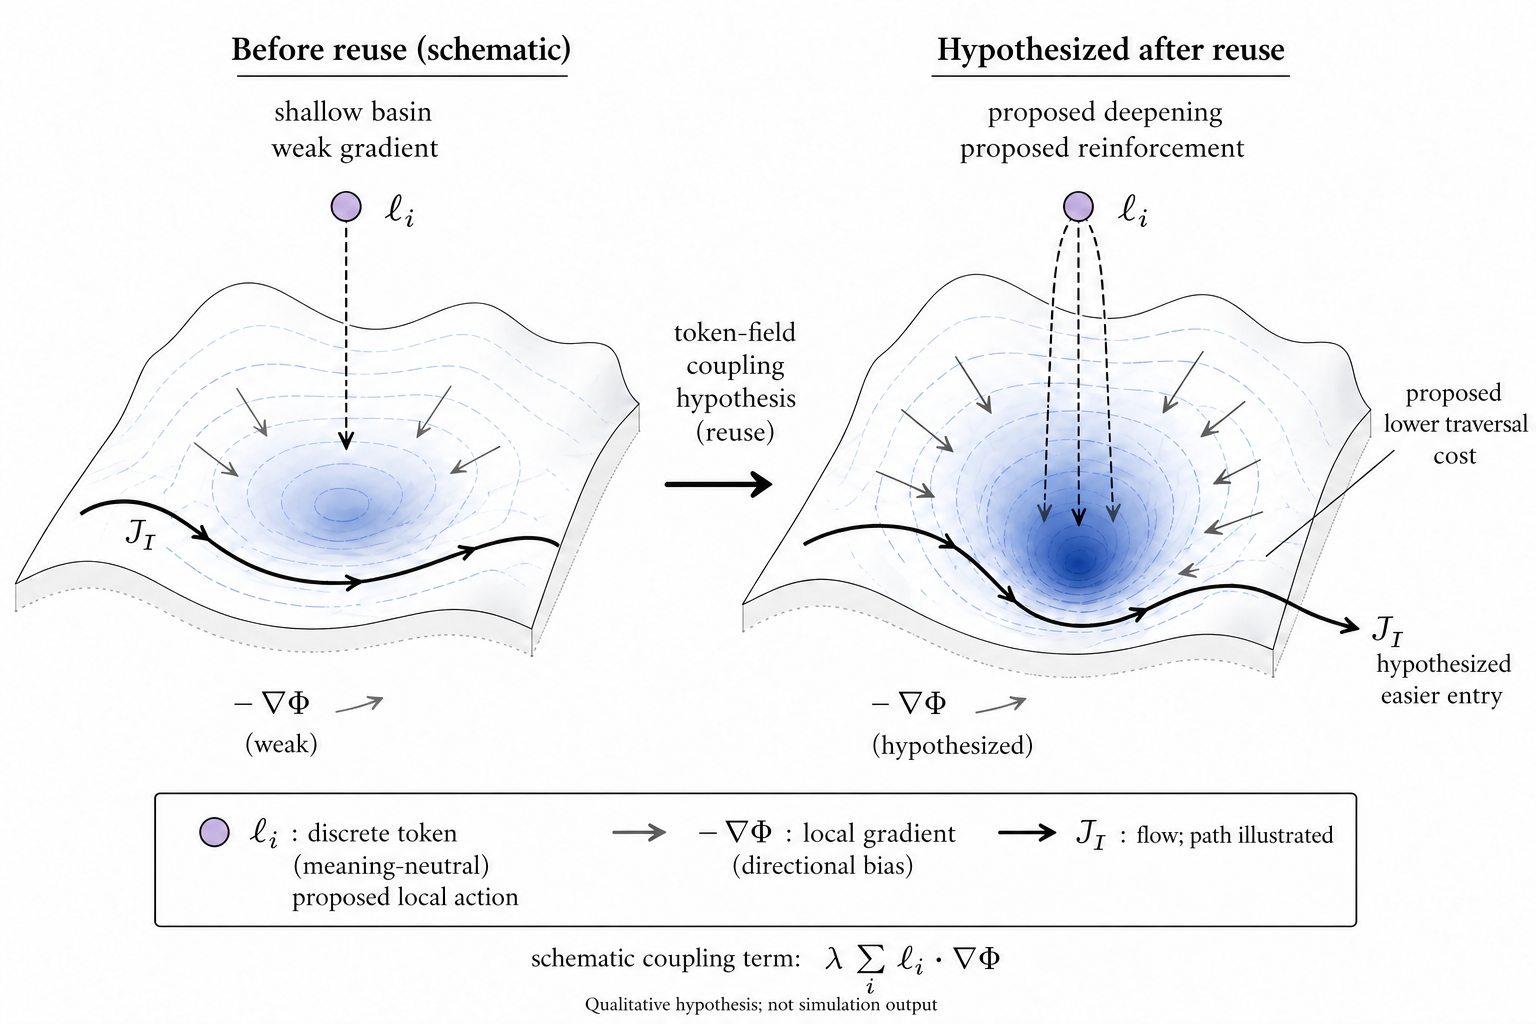
\includegraphics[width=0.95\linewidth]{figures/fig2_token_field_coupling.png}
\caption{
トークンと場の結合仮説の模式図であり、シミュレーション出力ではない。
離散トークン$\ell_i$には内在的な意味を割り当てず、$\nabla\Phi$への提案的な局所結合を動機として図示する。
$J_I$に関連する経路についての深化と通過コスト低下は仮説的効果であり、実行済みまたは導出済みの結果ではない。
表式$\lambda \sum_i \ell_i \cdot \nabla\Phi$は模式的なものに留まり、トークンの実現とペアリングは未解決である。
}
\label{fig:token-field-coupling}
\end{figure}

この構造を可能にする媒体は言語場である。
ここで「言語」は自然言語に限定せず、局所的な摂動として場に作用しうる、離散的で再アドレス可能なあらゆる媒体を広く含む。
記号、紋章、身振り、図、数式表記などが該当する。

言語トークン$\ell_i$（そのような任意の媒体から取られる離散単位）には、次の有効なトークン・場結合表式を割り当てる。
\begin{equation}
  \mathcal{L}_{\mathrm{eff}} = \mathcal{L}_{\mathrm{field}}[I]
  + \mathcal{L}_{\mathrm{token}}[\ell]
  + \lambda \sum_i \ell_i \cdot \nabla\Phi.
  \label{eq:coupling}
\end{equation}

提案する結合の役割は意味的なものではなく動的なものである。
トークンは意味を符号化せず、反復的な相互作用を通じて$\Phi$の局所的な発展に偏りを与えると仮定する。
勾配の強化と井戸の深化は定性的な機構仮説であり、項を書くだけで確立される帰結ではない。
結合表式は、離散トークンの数値的・ベクトル的実現と、ドット記法が示唆するペアリングに関して模式的なままであり、いずれも形式的には指定されていない。
有効・場・トークンの各ラグランジアン項の数学的な種類と、結合パラメータの仕様も未解決である。
ここでは、この表式からEuler--Lagrange方程式や、その他の変分・更新ダイナミクスを導出しない。

\subsection{沈殿と概念地形の形成}
以下の長時間表式は、反復的なトークンと場の相互作用の沈殿テンプレートとして保持し、確立された収束結果とはしない。
図\ref{fig:minimal-recursive-loop}は、枠組みの不可逆的順序という前提とともに、提案するフィードバック構成をまとめる。

\begin{figure}[t]
\centering
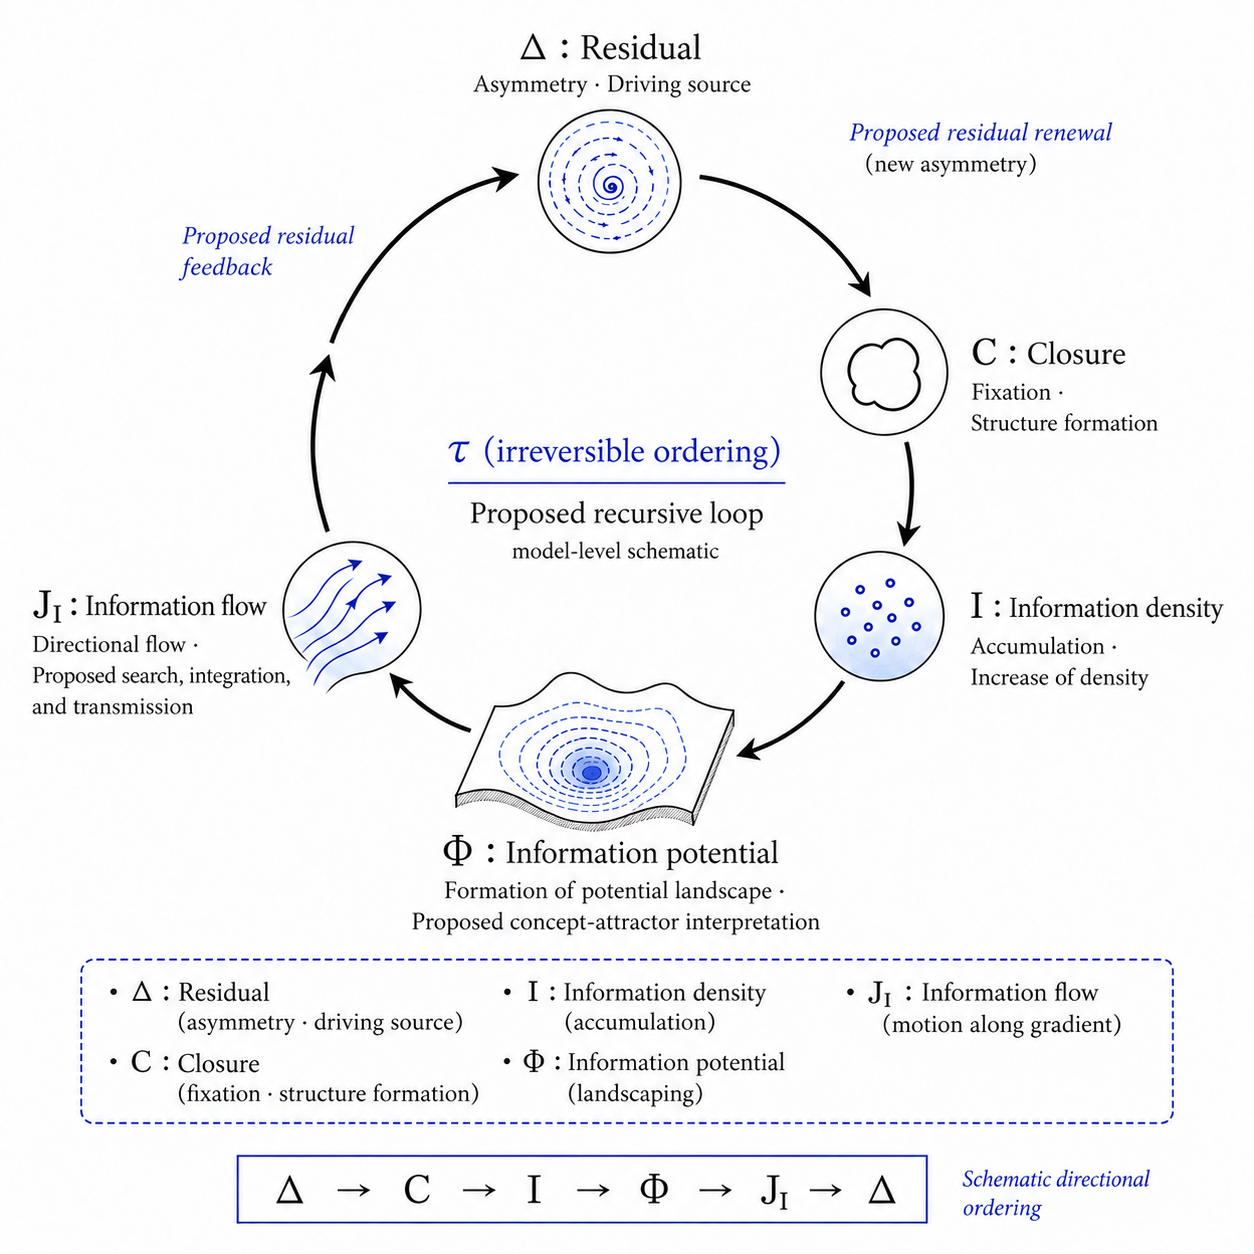
\includegraphics[width=0.82\linewidth]{figures/fig3_minimal_recursive_loop.png}
\caption{
VED$\times$IFGTの語彙による再帰ループの提案。
模式的な系列
$\Delta \to C \to I \to \Phi \to J_I \to \Delta$
は、残留非対称性$\Delta$、閉包$C$、情報密度$I$、ポテンシャル構造$\Phi$、情報流$J_I$を、提案するフィードバック構成の中で結びつける。
順序パラメータ$\tau$はモデルの不可逆的順序という前提を表す。
矢印は因果性の証明でも、実行された動的過程の実証でもない。
}
\label{fig:minimal-recursive-loop}
\end{figure}

\begin{equation}
  \Phi(x,\tau) \;\xrightarrow{\;\tau\to\infty\;}\; \Phistar(x).
  \label{eq:sedimentation}
\end{equation}

この矢印は長時間テンプレートであり、収束の様式は指定されていない。
以下の履歴解釈には、形式的な未解決性と出典・版に関する未解決性が残る。
表示された極限対象と、新たな入力による継続的な再形成との関係は、ここでは決定しない。
以下の非一意性・非静的性に関する表現は版に依存しており、その差を解消するために特定の解釈を選択しない。

$\Phistar$は沈殿した概念地形である。
それは必ずしも一意または静的ではなく、過去のすべての相互作用の履歴を反映し、新たな入力によって再形成され続ける。
ただし、地形が成熟するにつれてその速度は低下する。

\subsection{概念の定義}
\begin{definition}[概念]
位置$x$における\emph{概念}とは、次を満たす情報ポテンシャルの局所的安定領域である。
\begin{equation}
  \nabla\Phi(x) \approx 0, \qquad
  \text{with stability under small perturbations of } \JI.
  \label{eq:concept}
\end{equation}
$x$におけるポテンシャル井戸の深さには、変形への抵抗との構造的対応を提案する。
幅は文脈の広がりと比較する。これらの解釈は意味の較正ではない。
\end{definition}

\begin{definition}[理解]
概念領域$\mathcal{R}$を\emph{理解する}とは、$\mathcal{R}$を通る$\JI$の通過コストが、系に依存する閾値$\theta$より低くなっている状態である。
\begin{equation}
  \int_{\mathcal{R}} |\nabla\Phi|\,dx < \theta.
  \label{eq:understanding}
\end{equation}
ここで$\theta$は、再帰コストの許容範囲を表す、系に依存する有効閾値である。
具体的な値は$D$、$\mu$、$\alpha$および関連するパラメータを含む系の構造に依存し、本論文では指定しない。
理解は二値的な状態ではなく、$\Phi$の発展に伴って出入りしうる動的条件である。
\end{definition}

この定義は局所的なモデル状態を指定するものであり、独立した認知的・現象的基準ではない。
したがって、感じられる容易さとの提案的関係は別途評価しなければならない。
低コストな状態を定義することは、理解の経験を説明することではない。

\subsection{厳密な正値性制約}
厳密な正値性の記述は、モデルレベルの許容条件として保持する。
この正値域の制約、以下の正出力の前提、そして全収支発展のもとでの保存は、別々の形式的責務であり、ここではその正当化を確立していない。
この記述
\begin{equation}
  \boxed{I(x,\tau) > 0 \qquad \forall\,x,\,\tau,}
  \label{eq:positivity}
\end{equation}
は、$C < \Cmax$および$C < \Cmax$に対する正出力の前提$I = f(1-C) > 0$とともに述べられる。
ここで$\Cmax$は理想的な完全閉包境界を表し、概念系の通常の到達可能な状態ではない。

\begin{proposition}[通常の完全な概念的閉包の不在]
VED$\times$IFGTのモデル解釈内では、$I>0$は完全な概念的閉包を通常の動的状態から排する。
これとは別に、残留非対称性、空間的不均一性、境界構造を持つ非自明な地形では、$\Phi$のさらなる勾配と$\JI$の利用可能な方向が再び現れると提案する。
これは条件付きの分化仮説であり、正値性だけの帰結ではない。
閉包についての解釈は、正の$I$がすべて$\nabla\Phi\neq0$を持たねばならないという各点での数学的主張ではない。
追加条件なしでは、正値性だけから非ゼロの流れも含意されない。
完全な流れにはポテンシャル勾配の寄与以外も含まれる。
\end{proposition}

\begin{remark}
このモデルレベルの区別は、知性と理解との比較を動機づけるものであり、それらを正値性から導出するものではない。
安定アトラクタは局所的に静穏に見えることがある。
新たな摂動や、より広い観測窓のもとでは、さらなる分化が可能であり続けると提案する。
無条件の学習や革新の保証は推論しない。
\end{remark}
